%!TEX program = xelatex
\documentclass[11pt,a4paper]{article}

% -- Packages --
\usepackage[top=0.6in, bottom=0.6in, left=0.65in, right=0.65in]{geometry}
\usepackage{xeCJK}
\usepackage{fontspec}
\usepackage{titlesec}
\usepackage{enumitem}
\usepackage{hyperref}
\usepackage{xcolor}
\usepackage{graphicx}
\usepackage{tabularx}
\usepackage{fancyhdr}
\usepackage{tikz}
\usepackage{fontawesome}

% -- Fonts --
\setCJKmainfont[BoldFont=Noto Serif CJK SC Bold]{Noto Serif CJK SC}
\setCJKsansfont[BoldFont=Noto Serif CJK SC Bold]{Noto Serif CJK SC}
\setCJKmonofont{Noto Serif CJK SC}
\setmainfont{Noto Serif}[BoldFont=Noto Serif Bold, ItalicFont=Noto Serif Italic]
\setsansfont{Noto Serif}[BoldFont=Noto Serif Bold, ItalicFont=Noto Serif Italic]

% -- Colors --
\definecolor{primary}{RGB}{0, 79, 144}
\definecolor{accent}{RGB}{100, 100, 100}
\definecolor{lightgray}{RGB}{230, 230, 230}
\definecolor{darktext}{RGB}{40, 40, 40}

% -- Hyperlink --
\hypersetup{colorlinks=true, linkcolor=primary, urlcolor=primary}

% -- Section Formatting --
\titleformat{\section}{%
  \large\bfseries\color{primary}\sffamily%
}{}{0em}{}[\color{lightgray}\titlerule]
\titlespacing*{\section}{0pt}{10pt}{5pt}

% -- List Style --
\setlist[itemize]{leftmargin=1.2em, itemsep=1.5pt, parsep=0pt, topsep=3pt}

% -- Page Style --
\pagestyle{fancy}
\fancyhf{}
\renewcommand{\headrulewidth}{0pt}
\fancyfoot[C]{\small\textcolor{accent}{\thepage}}

% -- Custom Commands --
\newcommand{\cventry}[3]{%
  \vspace{6pt}
  \noindent{\textbf{\color{darktext}#1}} \hfill {\small\textcolor{accent}{#2}}\\[1pt]
  {\small\textcolor{accent}{#3}}
  \vspace{2pt}
}

\newcommand{\infoitem}[2]{\small{#1}\ {#2}}

% ==========================================
\begin{document}

% -- Top accent bar --
\noindent
\begin{tikzpicture}[remember picture, overlay]
  \fill[primary] (current page.north west) rectangle ([yshift=-3pt]current page.north east);
\end{tikzpicture}

\vspace*{-8pt}

% -- Header --
\noindent
\begin{minipage}[c]{0.20\textwidth}
  \centering
  \begin{tikzpicture}
    \clip circle (1.2cm);
    \node at (0,0) {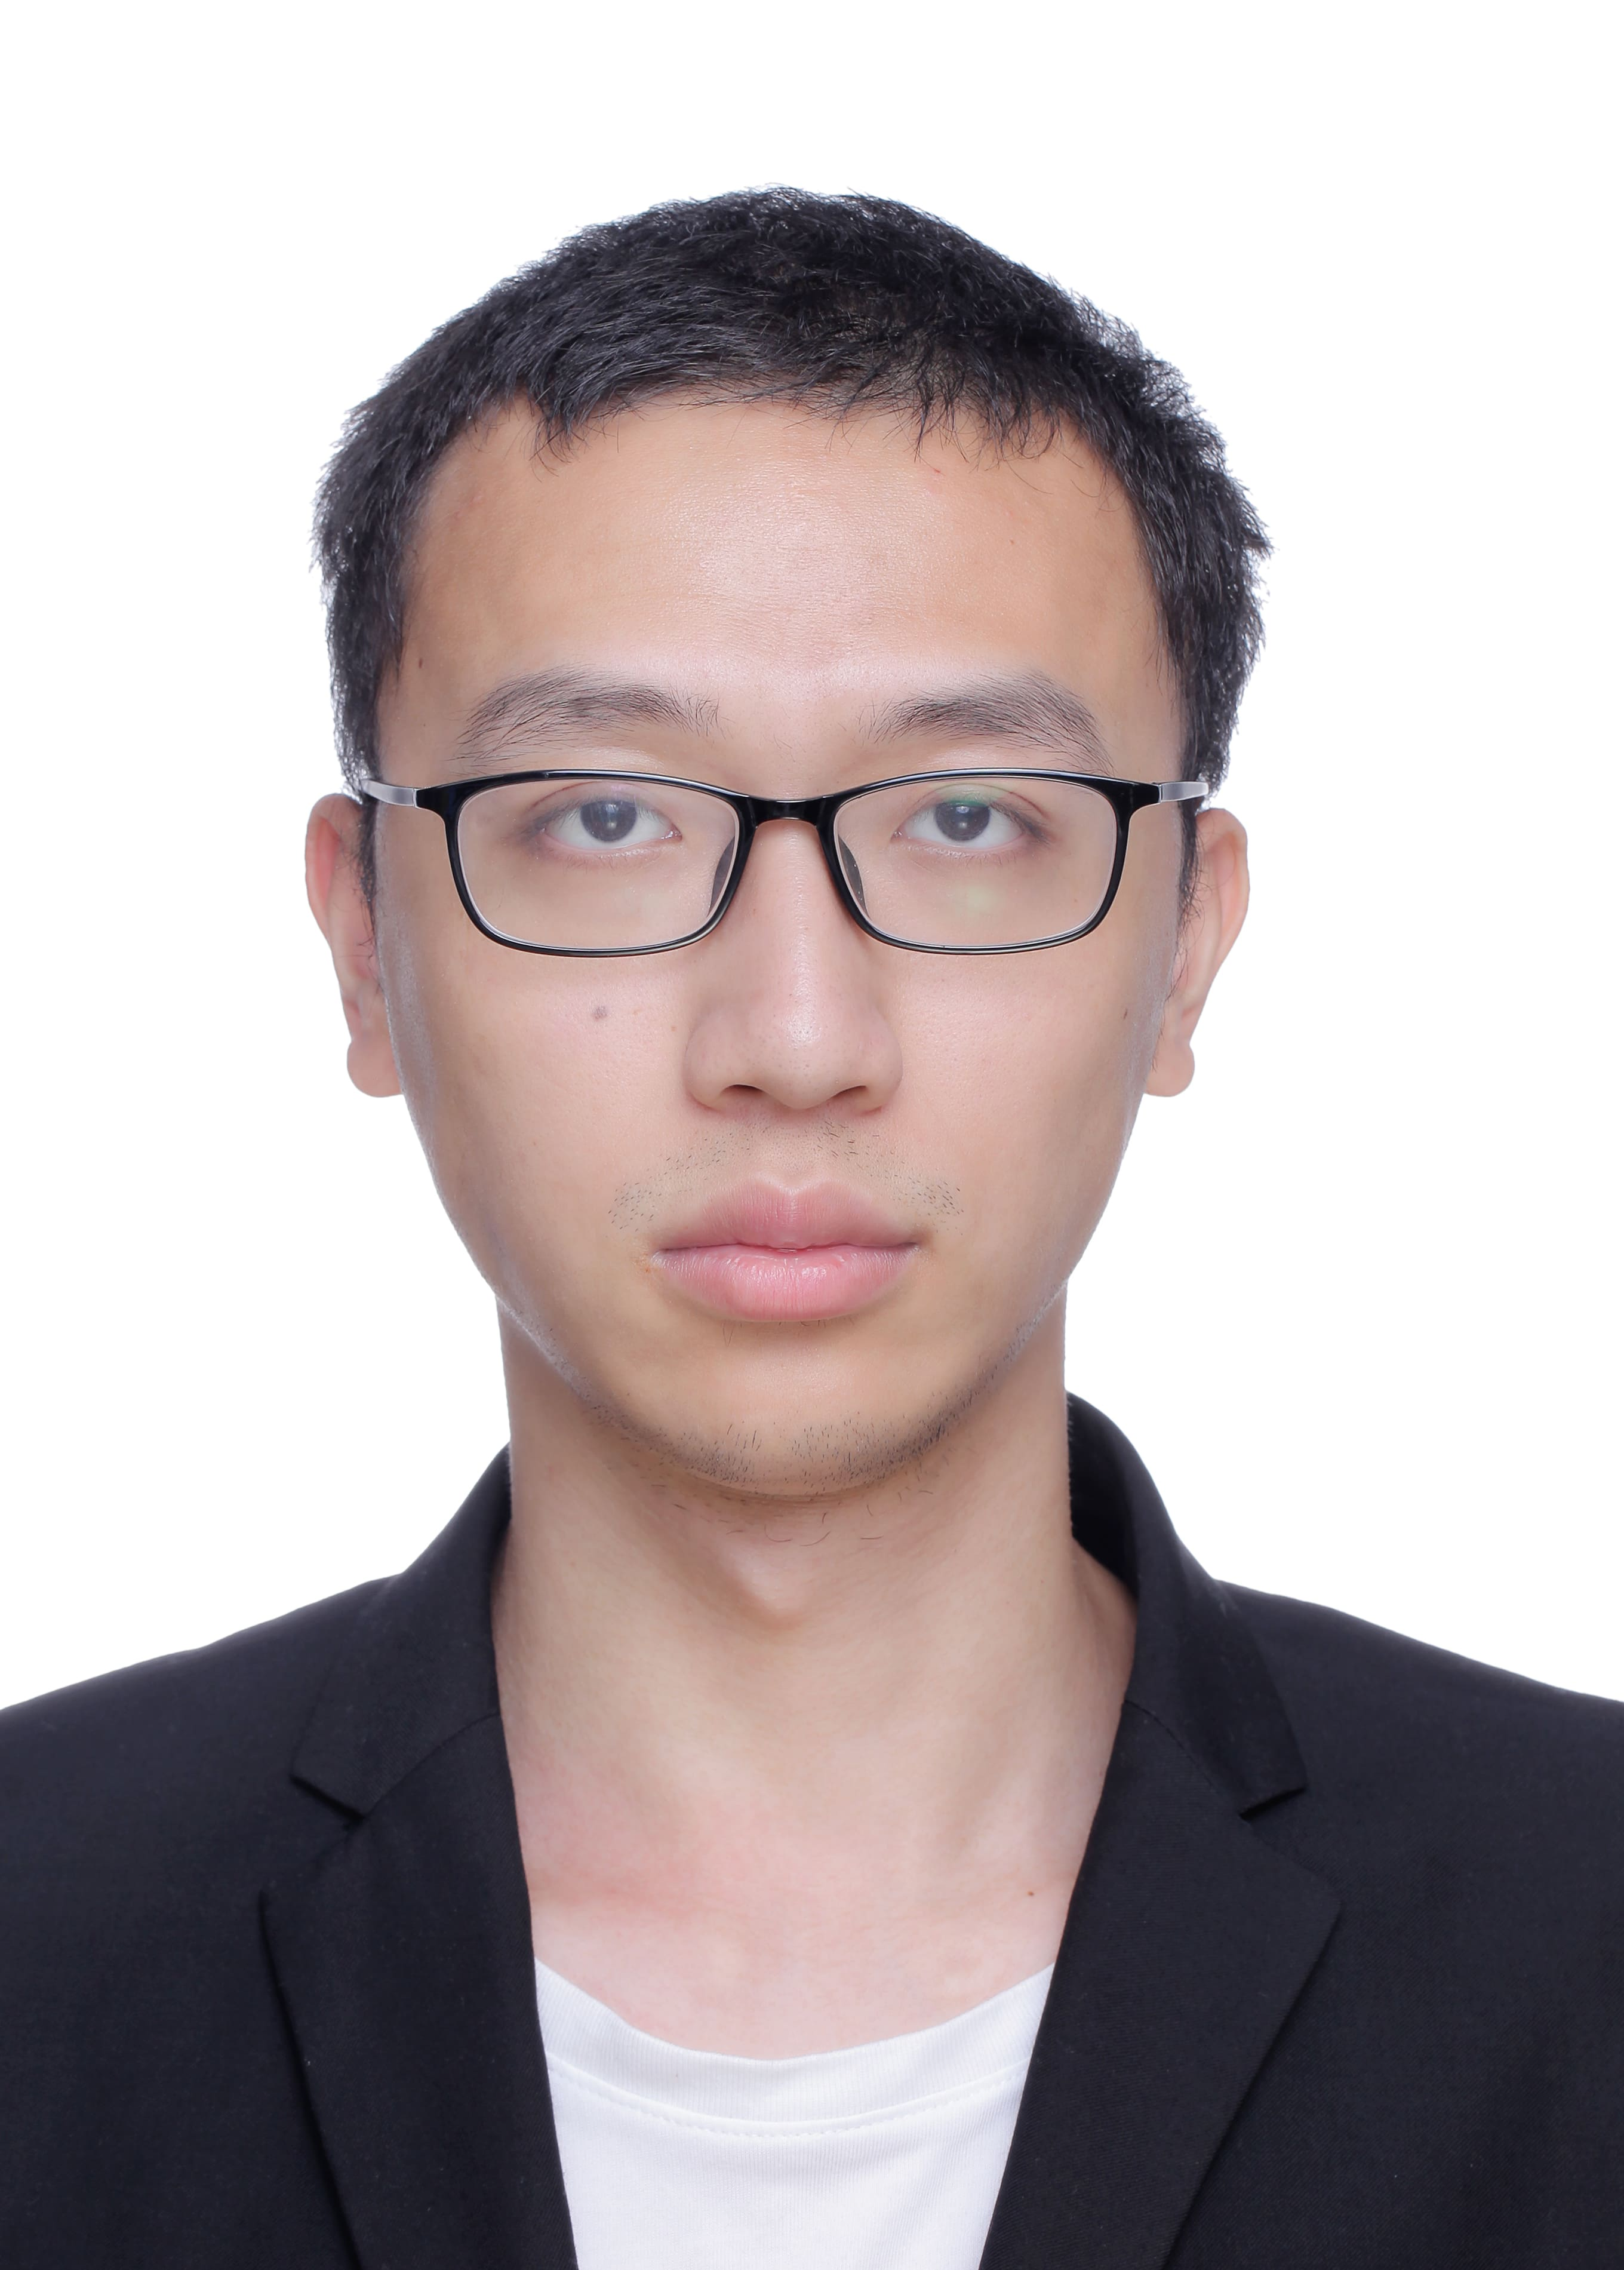
\includegraphics[width=2.4cm]{photo.jpg}};
  \end{tikzpicture}
\end{minipage}%
\hfill
\begin{minipage}[c]{0.78\textwidth}
  {\LARGE\bfseries\color{darktext}\sffamily Zhengyue Shao}\\[5pt]
  {\large\color{primary}\sffamily Software Engineer 2 \textperiodcentered{} Microsoft}\\[5pt]
  \infoitem{\faPhone}{17368941285} \quad
  \infoitem{\faEnvelope}{\href{mailto:419396971@qq.com}{419396971@qq.com}} \quad
  \infoitem{\faGithub}{\href{https://github.com/szylover}{szylover}} \quad
  \infoitem{\faGlobe}{\href{https://www.lovebxy.net}{lovebxy.net}}
\end{minipage}

\vspace{4pt}
\noindent{\color{lightgray}\rule{\textwidth}{0.5pt}}
\vspace{2pt}

{\small\color{accent}
Software Engineer with 8+ years at Microsoft, contributing to Android platform engineering, SDK/runtime design,
voice assistants, AI meeting experiences, and AI product integration. Experienced in client-side feature work,
host app integration, reliability improvements, and release support in cross-team projects.
}

% ==========================================
\section{\faBriefcase\quad Experience}

\noindent
{\large\bfseries\color{darktext}\sffamily Microsoft} \hfill {\small\textcolor{accent}{Software Engineer 2 \quad|\quad Jun 2017 -- Present}}

\cventry{M365 Copilot Mobile Runtime -- OCM}{2025 -- Present}
{Contribute to the Android SDK for OneCopilotMobile, shared by host apps including OfficeMobile, Outlook, and Teams.}
\begin{itemize}
  \item Support day-to-day OCM Android SDK engineering: releases, host integration support, cross-module compatibility, ECS rollout approvals, and feature flag management.
  \item Contribute to Copilot runtime infrastructure across configuration, feature gates, GPT-5 model switching, rich response rendering, and realtime voice integration.
  \item Implement assigned product and compliance modules including quote context injection, compliant WebSocket routing, and image upload consent flow.
\end{itemize}

\cventry{Outlook Android -- Search \& Compliance}{2024 -- 2025}
{Contributed to Outlook Android search experiences and security/compliance-related feature work.}
\begin{itemize}
  \item Outlook search module work: People, Files, and Events tab architecture, result rendering, and performance telemetry.
  \item Outlook Search page UX: custom search result rendering, search interactions, and page experience.
  \item Security and compliance modules: Intune enterprise policy checks, SafeLink integration, and resource access control fixes.
\end{itemize}

\cventry{Teams MeetApp -- AI Meeting Experience}{2022 -- 2024}
{Contributed to MeetApp in the Teams Windows Desktop React Native project, providing AI-enhanced meeting management experiences for Teams Desktop.}
\begin{itemize}
  \item Participated in MeetApp architecture design and feature development, including Graph/Substrate API clients, data pipeline, meeting list, Recap navigation, and AI summary features.
  \item Contributed to Copilot entry points and cross-meeting AI summaries, including BizChat streaming conversation flow.
  \item Helped build performance telemetry with Kusto/Augloop, debugging tools, and production investigations for issues such as memory leaks and navigation latency.
\end{itemize}

\cventry{Voice Assistants and Conversational AI -- Cortana / PME}{2019 -- 2022}
{Contributed to Android experiences for Play My Email, Catch Me Up, and Play My Messages.}
\begin{itemize}
  \item Contributed to Catch Me Up integration in Teams Android from POC to GA, covering React Native native bridge, Cortana voice interaction, KWS/AEC/TTS, and message triage actions.
  \item Developed streaming email readout and voice command handling in Outlook, with session reliability improvements for retry, network recovery, and state management.
  \item Participated in Hermes engine migration and SDX architecture refactoring, including support for Gov Cloud deployment.
\end{itemize}

\cventry{SharePoint Online -- Build Infrastructure}{2017 -- 2019}
{Worked on build system modernization for the large-scale SharePoint Online monorepo.}
\begin{itemize}
  \item Participated in migration from the legacy build system to Domino (BuildXL), improving incremental build workflows.
  \item Supported forward integration across branches and build break response as part of the DRI rotation.
\end{itemize}

% ==========================================
\section{\faGraduationCap\quad Education}

\cventry{Zhejiang University}{2014 -- 2017}{M.S. in Computer Science and Technology \quad Research: mobile security and BYOD access control}

\cventry{Nanjing University of Aeronautics and Astronautics}{2010 -- 2014}{B.S. in Computer Science and Technology \quad Admitted through NOIP First Prize recommendation, 2009}

% ==========================================
\section{\faBook\quad Publications}

\begin{itemize}[leftmargin=1.2em, itemsep=4pt]
  \item \textbf{RiskCog: Unobtrusive Real-Time User Authentication on Mobile Devices in the Wild}\\
    {\small T.~Zhu, Z.~Qu, H.~Xu, J.~Zhang, \textbf{Z.~Shao} et al. \quad
    \textit{IEEE Transactions on Mobile Computing}, 2019 \quad|\quad \textbf{92 citations}}

  \item \textbf{AppShield: Enabling Multi-entity Access Control Cross Platforms for Mobile App Management}\\
    {\small Z.~Qu, G.~Guo, \textbf{Z.~Shao} et al. \quad
    \textit{SecureComm 2016} (Springer LNCS) \quad|\quad \textbf{11 citations}}
\end{itemize}

% ==========================================
\section{\faCogs\quad Skills}

\begin{tabularx}{\textwidth}{@{} >{\bfseries\color{primary}\small}l >{\small}X @{}}
Android Platform & Kotlin, Java, Jetpack Compose, Coroutines/Flow, Dagger/Hilt, OkHttp/WebSocket, Room, React Native \\[3pt]
Architecture \& SDK & MVVM, Clean Architecture, SDK/runtime design, modularization, dependency injection, host/plugin architecture, feature gates \\[3pt]
AI Integration & Copilot integration, AI context pipeline, voice interaction (TTS/AEC/KWS), compliance UX, model switching \\[3pt]
Engineering & Monorepo CI/CD, build systems, performance telemetry/Kusto, staged rollout, production incident response, cross-team collaboration \\
\end{tabularx}

\end{document}
